\chapter{Datenselektion} \label{kap:datenselektion}
Dieses Kapitel beschreibt die notwendigen Schritte, um aus den Rohdaten des Detektors einen analysierbaren Datensatz (ein sog. NTupel) herzustellen. Wichtig ist dabei, den Datensatz von möglichst viel Untergrund zu bereinigen, ohne zu viele Signalereignisse zu verlieren. Die in dieser Arbeit verwendeten Daten entstammen Proton-Proton-Kollisionen und wurden im Jahre 2012 vom LHCb-Detektor bei einer Schwerpunktsenergie von $\sqrt{s} = 8\tera\electronvolt$ aufgenommen. Die integrierte Luminosität beträgt ca. $2\femto\barn^{-1}$. Von einem Mitarbeiter der Arbeitsgruppe wurden die Daten aufbereitet als NTupel zur Verfügung gestellt. Wesentliche Schritte bei der Erstellung waren die Rekonstruktion der Ereignisse mittels der Software \textsc{Brunel} sowie die Analyse mit dem Programm \textsc{DaVinci}. Bei Letzterer findet zur Reduzierung des Untergrunds eine Vorselektion statt, die Stripping genannt wird. Die Software selbst bietet für jeden Zerfallskanal entsprechende Sätze von Selektionskriterien an. In Kapitel \ref{kap:stripping} wird aufgelistet, welche für diese Analyse verwendet werden.

\section{Selektionskriterien}
Wie bereits erwähnt, erfolgt die Reduzierung des Untergrunds in mehreren Schritten, die im Folgenden erläutert werden.

\subsection{Trigger} \label{kap:trigger}
Den ersten Schritt bildet das Trigger-System, das schon während der Datennahme die Ereignisse sondiert. Der LHCb-Detektor verwendet dabei ein zweistufiges System: Der hardwarebasierte \glqq L0 Trigger\grqq\ reduziert die Ereignisrate von $40\mega\hertz$ auf $1\mega\hertz$. Im Anschluss folgt der zweiteilige, softwarebasierte \glqq High Level Trigger\grqq\ (HLT), der die Ereignisrate schlussendlich auf $2-3\kilo\hertz$ reduziert \cite{trigger}.

Es stehen für verschiedenste Bedürfnisse diverse sogenannte \glqq Triggerlines\grqq\ zur Verfügung. Die in dieser Analyse verwendeten Triggerlines entsprechen denen der Analyse der Daten aus 2011 \cite{lhcb-paper} und wurden wie folgt gewählt:

\subsubsection{High Level Trigger 1 (HLT1)}
Hier wird der \texttt{HltDiMuonHighMass} Trigger gewählt. Dieser rekonstruiert zwei Myonen, die einen gewissen Abstand zueinander haben, zu einem $J/\Psi$-Kan\-di\-da\-ten, dessen Masse eine gewisse Schwelle überschreiten muss. Bei der Selektion finden weiterhin die Qualität des $J/\Psi$-Vertex, die Myonen-Spuren sowie der (Transversal)Impuls des $J/\Psi$ Berücksichtigung.

\subsubsection{High Level Trigger 2 (HLT2)}
In dieser Analyse werden zwei unterschiedliche Linien verwendet. Zur Bestimmung der Detektorauflösung wird die \texttt{Hlt2\-DiMuon\-JPsi\-Decision} verwendet, die ähnliche Variablen wie beim HLT1 verwendet. Für die reguläre Analyse wird jedoch die \texttt{Hlt2\-DiMuon\-Detached\-JPsi\-Decision} verwendet, die zusätzlich die Signifikanz der Eigenzeit eines $J/\Psi$ berücksichtigt. Dadurch kommt es zu einer zeitabhängigen Nachweiseffizienz der \Bd-Mesonen. Der Vorteil dieser Triggerwahl liegt jedoch darin, dass mehr Statistik zur Verfügung steht und Untergrund massiv unterdrückt wird.

\subsection{Stripping} \label{kap:stripping}
Bei der Erstellung des Datensatzes wurde für das Stripping die Softwareversion DaVinci v32r2p1 (Stripping20r0p1) verwendet. Es wird nun aufgelistet, welche Selektionskriterien dabei angewandt wurden. Für die Auswahl des $\JPsi$ wurde auf die Selektion \texttt{Std\-Mass\-Constrained\-Jpsi\-2\-MuMu} zurückgegriffen, für das $\Kshort$ auf \texttt{StdLooseKsDD} sowie beim \Bd\ auf \texttt{Beta\-SBd2\-JpsiKs\-De\-tached\-Line} in der regulären Analyse bzw. \texttt{Beta\-SBd2\-JpsiKs\-Pre\-scaled\-Line} zur Bestimmung der Eigenzeitauflösung. Die in diesen Sätzen enthaltenen Selektionskriterien sind in Tabelle \ref{tab:cuts_stripping} aufgeführt.
\begin{table}[hptb]
\centering
\caption{Im Stripping verwendete Kriterien zur Selektion von \Bd, $\JPsi$ und $\Kshort$.}
\label{tab:cuts_stripping}
$\begin{array}{l|ll}
\hline \hline
\text{Zerfall} & \text{Variable} & \text{Wert} \\ \hline
$\Decaychannel$ & M($\Bd$) & \in [5150,5550] \mega\electronvolt \\
& \frac{\chi^2_{vtx}}{\text{nDof}}($\Bd$) & < 10 \\ \hline
\JPsi \rightarrow \mu^+\mu^- & \frac{\chi^2_{track}}{\text{nDof}}(\mu^{\pm}) & < 3 \\
& \Delta \ln \mathcal{L}_{\mu\pi} & > 0 \\
& p_T(\mu^{\pm}) & > 500 \mega\electronvolt\\
& \frac{\chi^2_{vtx}}{\text{nDof}}(\JPsi) & < 16 \\
& |M(\mu^+\mu^-)-M(\JPsi)| & < 80 \mega\electronvolt \\ \hline
\Kshort \rightarrow \pi^+\pi^- & p(\pi^{\pm}) & > 2000 \mega\electronvolt \\
& \frac{\chi^2_{vtx}}{\text{nDof}}(\Kshort) & < 20 \\
& \frac{\chi^2_{track}}{\text{nDof}}(\pi^{\pm}) & < 3 \\
& |M(\pi^+\pi^-)-M(\Kshort)| & < 64 \mega\electronvolt \\
& \frac{\chi^2_{IP}}{\text{nDof}}(\pi^{\pm}) & > 4 \\ \hline \hline
\end{array}$
\end{table}

In der Tabelle bezeichnen $M$ die rekonstruierte Masse, $p$ den Impuls sowie $p_T$ den Transversalimpuls eines Teilchens. Zur Rekonstruktion werden weiterhin Spuren an die Detektormessungen gefittet. Um eine Aussage über die Güte des Fits zu erhalten, betrachtet man hier das entsprechende auf die Zahl der Freiheitsgrade (nDoF) normierte $\chi_{track}^2$. Analog gilt dies für die Rekonstruktion der Vertices ($\chi_{track}^2$). Je näher das normierte\footnote{Synonym wird oft der Begriff \glqq reduziertes  $\chi^2$\grqq\ verwendet.} $\chi^2$ der 1 kommt, desto besser ist der Fit. IP steht für den Stoßparameter und $\Delta \ln \mathcal{L}_{\mu\pi}$ ist ein Maß für die Wahrscheinlichkeit, ein Myon als Pion zu interpretieren und umgekehrt. Ist der Wert größer als Null, so ist die Wahrscheinlichkeit, dass das Teilchen ein Myon ist größer, als diejenige, ein Pion zu sein.

\subsection{Verwendete Spurklassen} \label{kap:downstream}
Für die Rekonstruktion der $J/\Psi$ werden ausschließlich \glqq Long\grqq-Spuren verwendet. Diese passieren das gesamte Spurrekonstruktionssystem. Durch die relativ lange Lebensdauer des $\Kshort$ kommt es in etwa 2/3 der Fälle vor, dass die Zerfallsprodukte des $\Kshort$ nicht mehr in der Akzeptanz des VELO zerfallen und er in der Folge diese nicht mehr registriert. Hinterlassen Teilchen nur in den TT und T Stationen Spuren, so spricht man von \glqq Downstream\grqq-Spuren (siehe auch Kap. \ref{kap:spurklassen}). Diese Analyse beschränkt sich auf diese Spuren zur Rekonstruktion des $\Kshort$-Mesons. Damit hat man im Vergleich zu $\Kshort$ aus Long-Spuren mehr Statistik zur Verfügung, muss aber bei der Qualität der Rekonstruktion Einbußen hinnehmen, da die Informationen des VELO fehlen. Die Analyse der Long-Spuren ist Bestandteil einer anderen Bachelorarbeit. Bei Downstream-Spuren leidet insbesondere die Präzision der Impuls- und Positionsmessungen. Folglich dürfen die Selektionskriterien bei Downstream-Spuren teilweise nicht so hart sein wie bei Long-Spuren \cite{lhcb-paper}.

\subsection{Zusätzliche Selektionskriterien}
Um den Datensatz noch besser vom Untergrund zu bereinigen, werden einige Kriterien aus dem Stripping verschärft und weitere eingeführt (siehe Tab. \ref{tab:cuts_offline}). Diese wurden aus \cite{lhcb-paper} übernommen.
\begin{table}[hptb]
\centering
\caption{Zusätzlich eingeführte Kriterien zur Untergrundbereinigung bzw. Selektion von \Bd, $\JPsi$ und $\Kshort$.}
\label{tab:cuts_offline}
$\begin{array}{l|ll}
\hline \hline
\text{Zerfall} & \text{Variable} & \text{Wert} \\ \hline
$\Decaychannel$ & M($\Bd$) & \in [5170,5420] \mega\electronvolt \\
& \tau($\Bd$) & > 0,3\ps \\
& \sigma_\tau($\Bd$) & < 0,2\ps \\
& \frac{\chi^2_{DTF(B+PV)}}{\text{nDof}}($\Bd$) & < 5 \\
& \frac{\chi^2_{IP}}{\text{nDof}}($\Bd$) & < 20 \\ 
& \frac{\chi^2_{IP}}{\text{nDof}}($\Bd$) \text{ des nächstbesten PV} & > 50 \\ \hline
\JPsi \rightarrow \mu^+\mu^- & \frac{\chi^2_{vtx}}{\text{nDof}}(\JPsi) & < 11 \\
& |M(\mu^+\mu^-)-M(\JPsi)| & \in [3030,3165] \mega\electronvolt \\ \hline
\Kshort \rightarrow \pi^+\pi^- & \frac{\tau}{\sigma_\tau}(\Kshort) & > 5 \\
& \frac{l}{\sigma_l}(\Kshort) & > 5 \\
& |M(\pi^+\pi^-)-M(\Kshort)| & \in [475,520] \mega\electronvolt \\ \hline \hline
\end{array}$
\end{table}
Die neu eingeführten Größen sind hier die Eigenzeit $\tau$ und die Flugstrecke $l$ sowie deren Unsicherheiten $\sigma_\tau$ und $\sigma_l$. Weiterhin gibt es noch einen kinematischen Fit des gesamten Zerfallsprozesses (\glqq DecayTreeFit\grqq - DTF). Um die Wirkung der einzelnen Zusatzkriterien im Vergleich zum Stripping zu untersuchen, werden alle bis auf das zu untersuchende Kriterium angewandt und in der Massenverteilung das Signal-zu-Untergrund-Verhältnis $S/B$ bestimmt. Als Parametrisierung für den Fit der Massenverteilung wird ein doppelter Gauß verwendet, der Untergrund wird durch eine Exponentialfunktion modelliert (mehr dazu in Kap. \ref{kap:massenfit}). Zur Berechnung des Signals und des Untergrundes werden der Doppelgauß bzw. die Exponentialfunktion im Bereich von $\pm 3\sigma$ um den Mittelwert ausgewertet. Des Weiteren ist es von Interesse wie viel Signal und wie viel Untergrund man durch das entsprechende Kriterium verliert. Dazu werden die Verhältnisse $\epsilon_{\text{sig}}$ ($\epsilon_{\text{bkg}}$) von Signal (Untergrund) bei Anwendung aller Kriterien zu Signal (Untergrund) ohne ebenjenes Kriterium berechnet. Die Ergebnisse dieser Berechnungen sind in Tabelle \ref{tab:cuts_efficiency} aufgeführt.
\begin{table}[hptb]
\centering
\caption{Berechnung des Signal-zu-Untergrund-Verhältnisses $S/B$ sowie der Effizienzen $\epsilon_{\text{sig}}$ für Signal und $\epsilon_{\text{bkg}}$ für Untergrund.}
\label{tab:cuts_efficiency}
$\begin{array}{l|ccc}
\hline \hline
\text{ausgelassenes Kriterium} & S/B & \epsilon_{\text{sig}} & \epsilon_{\text{bkg}}\\ \hline
M($\Bd$) \in [5170,5420] \mega\electronvolt & 4,24 & 1,000 & 1,000 \\
\tau($\Bd$) > 0,3\ps & 2,71 & 0,955 & 0,610\\
\sigma_\tau($\Bd$) < 0,2\ps & 4,24 & 1,000 & 1,000 \\
\frac{\chi^2_{DTF(B+PV)}}{\text{nDof}}($\Bd$) < 5 & 3,58 & 0,984 & 0,831 \\
\frac{\chi^2_{IP}}{\text{nDof}}($\Bd$) < 20 & 3,67 & 0,992 & 0,860 \\ 
\frac{\chi^2_{IP}}{\text{nDof}}($\Bd$) \text{ des nächstbesten PV} > 50 & 3,50 & 0,979 & 0,809 \\ 
\frac{\chi^2_{vtx}}{\text{nDof}}(\JPsi) < 11 & 4,19 & 0,995 & 0,982\\
|M(\mu^+\mu^-)-M(\JPsi)| \in [3030,3165] \mega\electronvolt & 4,05 & 0,997 & 0,953\\ 
\frac{\tau}{\sigma_\tau}(\Kshort) > 5 & 4,18 & 0,995 & 0,982\\
\frac{l}{\sigma_l}(\Kshort) > 5 & 4,24 & 1,000 & 1,000 \\
|M(\pi^+\pi^-)-M(\Kshort)| \in [475,520] \mega\electronvolt & 3,37 & 0,985 & 0,782\\ \hline
\text{alle angewandt} & 4,24 & 1,000 & 1,000 \\ \hline \hline
\end{array}$
\end{table}
Am Beispiel der Selektion der Eigenzeit $\tau(\text{\Bd})$ soll noch einmal deutlich gemacht werden, wie die Tabelle zu lesen ist: Im Vergleich zur Anwendung aller Kriterien ($S/B=4,24$) ist das Signal-zu-Untergrund-Verhältnis ohne die Selektion anhand der Eigenzeit mit 2,71 deutlich schlechter. Während dieses Kriterium von 95,5\% des Signals passiert wird, ist dies nur bei 61,0\% des Untergrunds der Fall. Damit wird man fast 40\% des Untergrunds los, ohne $\epsilon_{\text{sig}}$ Signal wegzuwerfen. Anhand der Werte in Tabelle \ref{tab:cuts_efficiency} sieht man, dass dieses Kriterium das effektivste ist. Bei drei der Kriterien sieht man keine Änderung im Vergleich zur Anwendung aller Kriterien. Bei der weiteren Einschränkung der \Bd-Masse ist dies nicht weiter verwunderlich, da sich die Form der Massenverteilung nicht ändert, sondern nur an den Rändern abgeschnitten wird. Die Selektionen auf $\sigma_\tau($\Bd$)$ und $\frac{l}{\sigma_l}(\Kshort)$ sind nur schwache Kriterien, die zwar minimal selektieren, dies bei der angegebenen Genauigkeit aber nicht sichtbar wird. An dieser Stelle soll betont werden, dass man aus Tabelle \ref{tab:cuts_efficiency} nicht generell schließen kann, welche Kriterien sehr effektiv sind und welche man eigentlich gar nicht benötigt. Hierzu bedürfte es eines Vergleiches der Kriterien mit dem Datensatz vor dem Stripping. Dieses stand leider nicht zur Verfügung, sodass nur der relative Vergleich der Zusatzkriterien mit dem Datensatz nach dem Stripping gemacht werden konnte, sodass manche Kriterien, bei denen es mengenmäßige Überschneidungen mit Kriterien im Stripping gibt, als unnötig erscheinen.

\subsubsection{Bester Kandidat}
Es ist äußerst unwahrscheinlich, dass es mehrere \Decaychannel-Zerfälle in einem Ereignis gibt. Jedoch kann es vorkommen, dass es mehr als ein rekonstruiertes \Bd\ im Ereignis gibt. Da aber nur ein \Bd\ am Zerfall beteiligt ist, wird der beste Kandidat anhand des kleinsten $\chi^2_{DTF}/\text{nDoF}$ des DecayTreeFit identifiziert \cite{lhcb-paper}.

\subsubsection{Geisterspuren}
Für die Daten aus 2012 gibt es ein neues Kriterium, das in der Analyse der 2011 Daten \cite{lhcb-paper} noch nicht zur Verfügung stand und deshalb hier gesondert betrachtet wird: Die Analysesoftware gibt nun für die Pionen- und Myonenspuren eine Wahrscheinlichkeit an, dass es sich bei dieser Spur nur um eine Geisterspur handelt. Dies bedeutet, dass der Spurrekonstruktionsalgorithmus diversen Detektormessungen eine Spur zuordnet, die nichts miteinander zu tun haben. Bei der Suche nach einer Schranke für dieses Kriterium wurde 0,5 gewählt, denn ist die Wahrscheinlichkeit kleiner als 0,5, dann ist es wahrscheinlicher, dass es sich auch wirklich um eine Spur handelt, als dass es eine Geisterspur ist.

Wendet man dieses Kriterium auf Myonen an, so erhält man die Effizienzen $\epsilon_{\text{sig}}=0,999$ und $\epsilon_{\text{bkg}}=0,978$. Damit ist es bei Weitem nicht so effektiv wie beispielsweise die Eigenzeitselektion, leistet aber dennoch einen Beitrag zur Bereinigung des Datensatzes. Im Falle von Pionen kommt es zu Problemen. Eine Schranke bei 0,5 führt hier zu $\epsilon_{\text{sig}}=0,660$ und $\epsilon_{\text{bkg}}=0,561$. Leider geht deutlich zu viel Signal verloren. Es hat sich zudem herausgestellt, dass bei \glqq Downstream-Pionen\grqq\ die Wahrscheinlichkeitsberechnung in der Analysesoftware nicht korrekt kalibriert wurde und notwendige Korrekturen bei der Erstellung dieses Datensatzes nicht berücksichtigt wurden. Daher sind die zur Verfügung gestellten Werte nicht aussagekräftig und auf eine Selektion mittels der Geisterspur-Wahrscheinlichkeit eines Pions wird verzichtet.

\subsubsection{Fitbereiche}
In den Analysen werden beim Fit die Massenbereiche zusätzlich eingeschränkt. Zur Bestimmung der Detektorauflösung werden $\JPsi$ im Bereich $[3035, 3160]\mega\electronvolt$ betrachtet, im regulären Fit werden nur \Bd-Kandidaten im Bereich \linebreak$[5230, 5330]\mega\electronvolt$ berücksichtigt.

\section{Verfügbare Statistik}
Nach Anwendung aller Selektionskriterien stehen insgesamt 62184 Signalkandidaten zur Verfügung. Für diese Analyse ist essentiell, dass der Flavour der Mesonen (\Bd, \Bdbar) zum Zeitpunkt $t=0$ bekannt ist. Hierzu gibt es entsprechende Algorithmen, denen es gelingt, 20109 Signalkandidaten einen Anfangsflavour zuzuordnen. Dieser Prozess wird auch \glqq Favour Tagging\grqq\ genannt. Mehr dazu findet sich in Kapitel \ref{kap:tagging}. Die Zahl der Signalkandidaten wurde mit Hilfe eines Fits an die rekonstruierte \Bd-Masse bestimmt (siehe Kap. \ref{kap:massenfit}), dessen Ergebnis in Abbildung \ref{fig:masse_allein} dargestellt ist.
\begin{figure}[hptb]
\centering
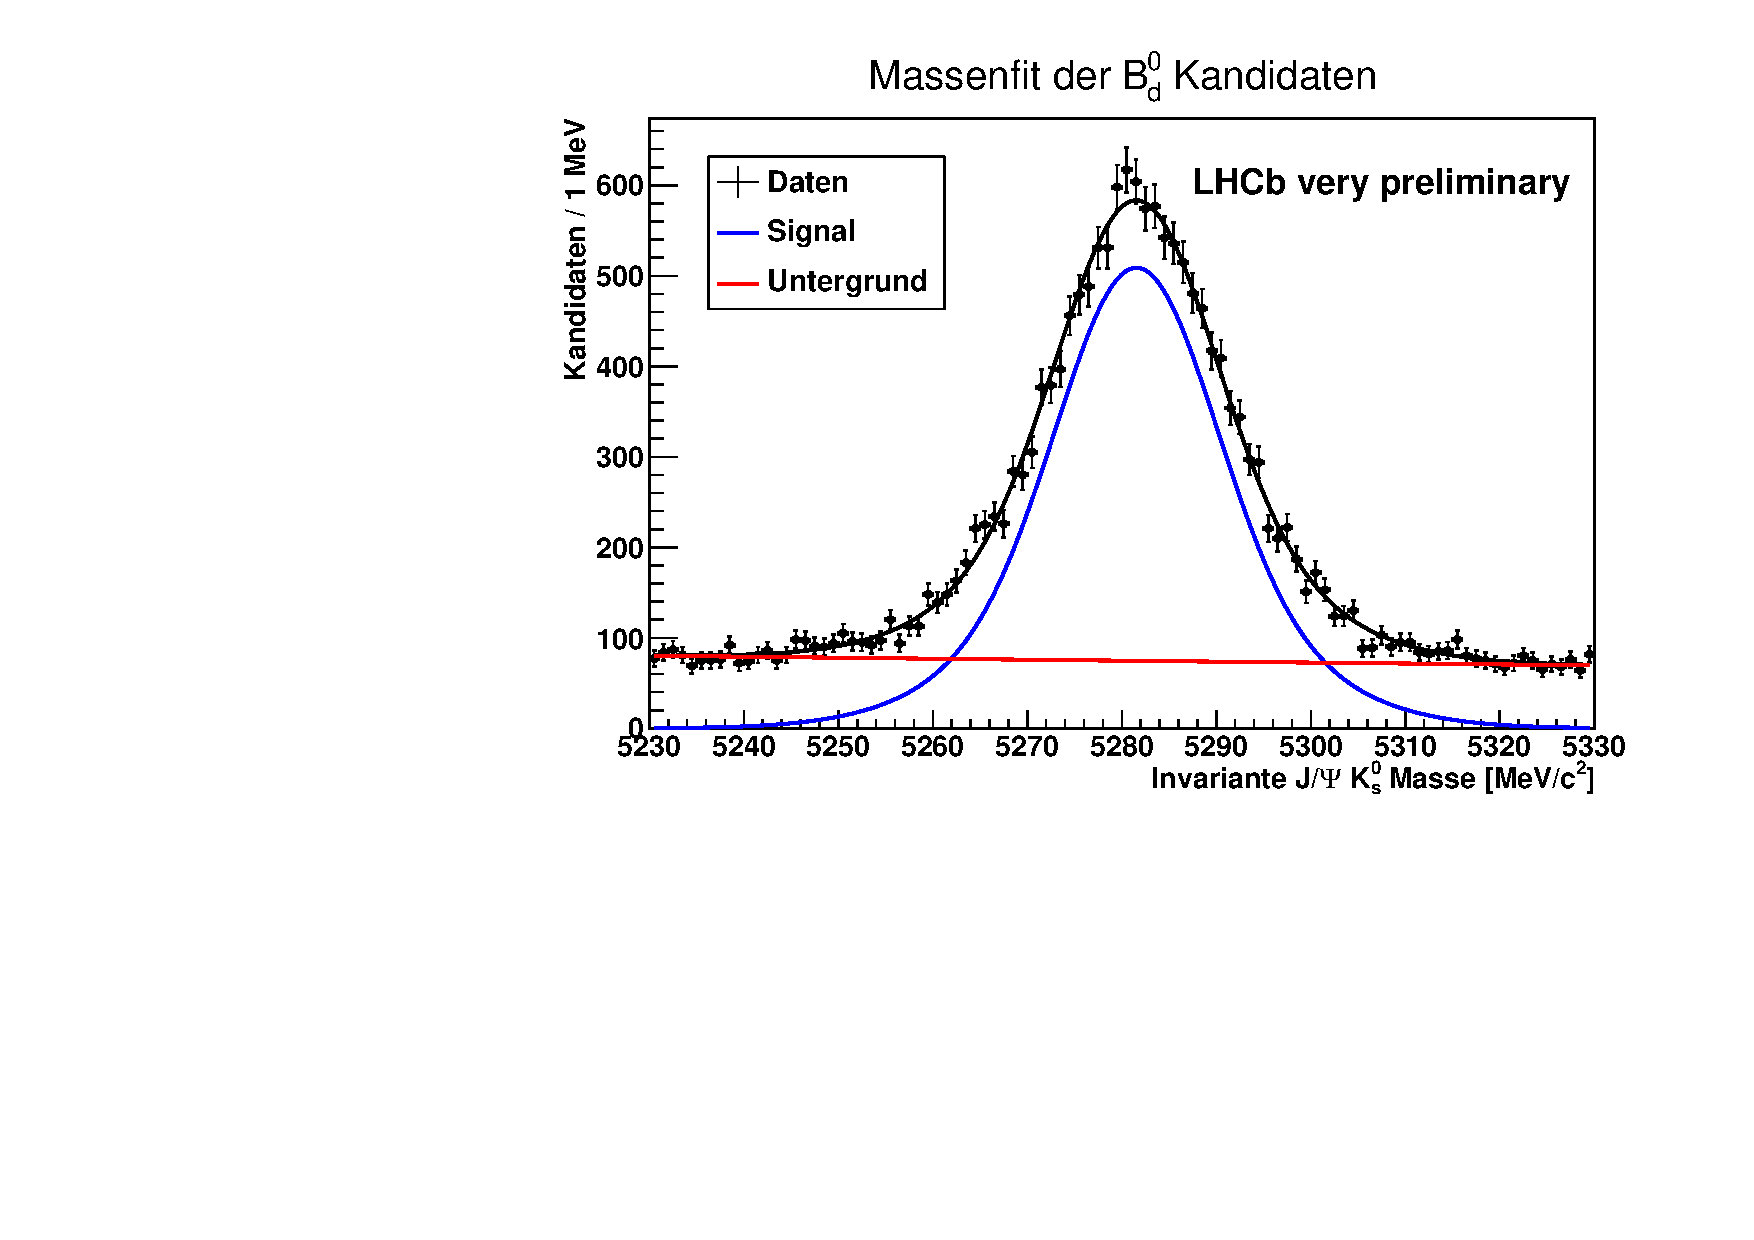
\includegraphics[width=\textwidth]{masse_allein}
\caption{Fit der rekonstruierten \Bd-Masse zur Bestimmung der Zahl an Signalkandidaten. Detaillierte Ergebnisse finden sich in Kapitel \ref{kap:massenfit}.}
\label{fig:masse_allein}
\end{figure}